\documentclass{article}
\usepackage{amsmath}
\usepackage{amssymb}
\usepackage{array}
\usepackage{algorithm}
\usepackage{algorithmicx}
\usepackage{algpseudocode}
\usepackage{booktabs}
\usepackage{colortbl}
\usepackage{color}
\usepackage{enumitem}
\usepackage{fontawesome5}
\usepackage{float}
\usepackage{graphicx}
\usepackage{hyperref}
\usepackage{listings}
\usepackage{makecell}
\usepackage{multicol}
\usepackage{multirow}
\usepackage{pgffor}
\usepackage{pifont}
\usepackage{soul}
\usepackage{sidecap}
\usepackage{subcaption}
\usepackage{titletoc}
\usepackage[symbol]{footmisc}
\usepackage{url}
\usepackage{wrapfig}
\usepackage{xcolor}
\usepackage{xspace}
\usepackage[utf8]{inputenc}
\usepackage{lipsum}

\title{Research Report: A Comprehensive Analysis of SPR-Based Sequence Recognition}
\author{Agent Laboratory}
\date{}

\begin{document}

\maketitle

\begin{abstract}
In this work, we address the challenging problem of sequence recognition in SPR tasks, where sequences composed of tokens with distinct shapes and colors require the identification of latent patterns critical for accurate classification; specifically, our approach extracts features by computing the number of unique shapes, unique colors, and total tokens per sequence, yielding a feature vector $\mathbf{x} \in \mathbb{R}^3$ that is input to a logistic regression model defined as $\hat{y} = \sigma(W\mathbf{x} + b)$, with $W \in \mathbb{R}^{1 \times 3}$ and $b \in \mathbb{R}$, while the nonuniform interactions among token features render this task intrinsically hard. Our experiments on the SPR\_BENCH dataset reveal that the baseline model achieves a standard accuracy of 59.14\%, a Shape-Weighted Accuracy (SWA) of 0.5857 and a Color-Weighted Accuracy (CWA) of 0.5745 on the development set, with the performance dropping on the test set to 54.25\%, 0.5411 and 0.5405 respectively, as summarized in Table~1, thereby indicating that the simple feature set fails to fully capture the underlying structure of the sequences. Our primary contribution is the establishment of this quantitative baseline, which highlights the necessity for enhanced feature extraction methodologies and non-linear modeling techniques to better infer the hidden target rules, and paves the way for future extensions such as incorporating interaction terms and neural-symbolic frameworks to move towards a target Closed-loop Weighted Accuracy of 65.0\%; these insights are further corroborated by rigorous evaluations using equations like $\hat{y} = \sigma(W\mathbf{x} + b)$ and associated performance metrics.
\end{abstract}

\section{Introduction}


\section{Background}
In many symbolic pattern recognition (SPR) tasks, the goal is to extract meaningful information from sequences of tokens where each token is associated with attributes such as shape and color. Early work in symbolic extraction has demonstrated that even simple feature counts can provide insight into abstract representations (arXiv 1710.00077v1). Building on these ideas, our background framework establishes a formal setting in which each input sequence is represented by a feature vector derived from counts of unique shapes, unique colors, and overall token count. Such feature vectors are fundamental to the subsequent application of linear classifiers, where a model of the form 
\[
\hat{y} = \sigma(W\mathbf{x} + b)
\]
is employed, with \(\mathbf{x} \in \mathbb{R}^3\), \(W \in \mathbb{R}^{1 \times 3}\), and \(b \in \mathbb{R}\). In this context, the non-linear activation \(\sigma\) (typically the logistic function) enables the transformation of the linear combination into a probabilistic output, laying the groundwork for statistical performance metrics such as standard accuracy.

A key component of this framework is the formal problem setting and notation. Let \(S = \{s_1, s_2, \ldots, s_n\}\) denote an ordered sequence of tokens, where each \(s_i\) is associated with a shape and a color. We define the feature extraction function \(f\) such that the feature vector is given by 
\[
\mathbf{x} = f(S) = \Bigl[ \#\{\text{unique shapes in } S\}, \; \#\{\text{unique colors in } S\}, \; \text{total token count} \Bigr]^\top.
\]
The adoption of this feature mapping allows us to abstract away from the raw symbolic content and focus on structural properties that are believed to underlie the SPR tasks. Assumptions inherent to this approach include invariance to the ordering of similar tokens and the stability of abstract features under token transformations. Performance metrics observed in preliminary experiments—such as a standard accuracy of 59.14\% on development datasets—underscore the challenges in capturing the full latent structure with such simple abstractions.

The background literature also emphasizes the transition from rigid symbolic methods to more flexible, non-linear approaches capable of modeling complex interactions between tokens. Recent studies (e.g., arXiv 2503.04900v1) have demonstrated the potential of self-supervised learning for extracting symbolic sequences from visual representations, thereby providing a complementary paradigm to classical symbolic pattern matching. A concise summary of our notations and assumptions is provided in Table~\ref{tab:notations} below:
\[
\begin{array}{|c|c|}
\hline
\textbf{Symbol} & \textbf{Description} \\
\hline
S & \text{Ordered sequence of SPR tokens} \\
\hline
\mathbf{x} & \text{Feature vector in } \mathbb{R}^3 \text{, where } \mathbf{x} = f(S) \\
\hline
W, \, b & \text{Parameters of the logistic regression model} \\
\hline
\hat{y} & \text{Predicted label given by } \sigma(W\mathbf{x} + b) \\
\hline
\end{array}
\]
This formal overview provides the necessary academic foundation and context, highlighting the evolution in approaches from basic feature counting to advanced neural-symbolic models. Such a progression is critical for understanding how improvements in SPR tasks are being engineered to bridge the gap between simple linear models and more sophisticated architectures that can better capture and exploit the inherent compositional structure of symbolic sequences.

\section{Related Work}
Recent work in the literature has focused on leveraging symbolic pattern matching and term rewriting systems to address sequence recognition problems. Approaches such as those presented in (arXiv:1710.00077v1) and (arXiv:1710.06915v1) employ explicit syntactic pattern matching, where input sequences are transformed into abstract representations using predefined rewrite rules. These methods typically use a formulation of the form 
\[
\hat{y} = W \, \phi(x) + b,
\]
with \(\phi(x)\) representing a manually crafted feature map that extracts symbolic attributes from the input. Although these systems benefit from a high degree of interpretability and formal guarantees under strict structural assumptions, they require substantial expert intervention to design appropriate rewriting rules. Moreover, the rigidity of these rules often limits their scalability to problems such as SPR tasks, where the interplay of token-based features such as shape and color introduces variability that the fixed symbolic rules may fail to capture. In practice, the performance of these methods generally suffers when confronted with sequences that deviate from the assumed regular patterns, as illustrated by achieved accuracies and shape-weighted accuracies that are frequently below the 60\% threshold.

In contrast, recent trends have shifted towards the use of deep non-linear architectures that inherently model complex interactions between sequence elements. For instance, frameworks discussed in (arXiv:2505.23833v1) propose deep neural networks structured as
\[
\hat{y} = \text{ReLU}(W_2\, \text{ReLU}(W_1 x + b_1) + b_2),
\]
which enable the model to learn hierarchical features from raw representations without the need for finely-tuned manual feature design. These models, while demonstrating strong performance in capturing non-linear dependencies, often require large training datasets and significant computational resources. Furthermore, despite their high expressivity, such deep models introduce challenges in interpretability—a crucial aspect when analyzing the latent compositional structure in SPR tasks. The divergence in methodology is further clarified by comparing the computational overhead and resultant performance. A summary of these differences is provided in Table~\ref{tab:compare}.

\begin{center}
\begin{tabular}{|l|c|c|}
\hline
\textbf{Method} & \textbf{Assumptions} & \textbf{SPR Applicability} \\
\hline
Symbolic Pattern Matching (e.g., arXiv:1710.00077v1) & Predefined rewrite rules; explicit syntactic structure & Limited by manual rule specification and rigidity \\
\hline
Deep Neural Architectures (e.g., arXiv:2505.23833v1) & High-capacity non-linear transformations; learned hierarchical features & Higher resource demand; less interpretable \\
\hline
Baseline Logistic Regression & Count-based features; linear separability & Direct and interpretable but limited in capturing complex interactions \\
\hline
\end{tabular}
\end{center}

Overall, these studies underline a fundamental trade-off between model interpretability and representational capacity. While symbolic methods offer clarity and explicit rule derivation, they do not easily extend to tasks requiring flexible generalization. Conversely, deep learning approaches achieve impressive accuracy by modeling sophisticated non-linear interactions, yet they often obscure the underlying decision process. Our current work situates itself at this intersection by using a simple logistic regression approach that, despite its limitations, provides a computationally efficient and interpretable baseline for SPR tasks. This comparison not only highlights the strengths and weaknesses of each paradigm but also motivates the need for future hybrid models that integrate the robustness of deep feature learning with the clarity of symbolic reasoning.

\section{Methods}
We adopt a feature extraction methodology that leverages the formalism introduced in the Background section, where each input sequence \(S\) is represented by a three-dimensional feature vector:
\[
\mathbf{x} = f(S) = \begin{bmatrix} \#\{\text{unique shapes in } S\} \\ \#\{\text{unique colors in } S\} \\ \text{total token count in } S \end{bmatrix} \in \mathbb{R}^3.
\]
The extracted features serve as the input to a logistic regression model defined by
\[
\hat{y} = \sigma(W\mathbf{x} + b),
\]
with \(W \in \mathbb{R}^{1 \times 3}\) and \(b \in \mathbb{R}\). The activation function \(\sigma\), typically implemented as the logistic function, transforms the linear combination into a probability estimate. Parameters \(W\) and \(b\) are estimated by minimizing the standard cross-entropy loss function:
\[
L = -\sum_{i=1}^{N}\left[y_i \log(\hat{y}_i) + (1-y_i)\log(1-\hat{y}_i)\right],
\]
where \(N\) denotes the number of training examples, and \(y_i\) represents the ground-truth label of the \(i\)-th example.

To evaluate our model rigorously, we compute several performance metrics including the standard classification accuracy, as well as the Shape-Weighted Accuracy (SWA) Color-Weighted Accuracy (CWA), defined so as to account for the complexity of the input sequence based on the diversity of its shapes and color, respectively. Empirical results on the SPR\_BENCH dataset indicate that the model achieves a standard accuracy of 59.14\%, an SWA of 0.5857 and a CWA of 0.5745 on the development set, with corresponding reductions to 54.25\%, 0.5411 and 0.5405 on the test set. The histogram of unique shape counts, presented in Figure~\ref{fig:fig1}, provides insight into the variability of shape diversity across the training sequences.

\begin{figure}[h]
\caption{Histogram of unique shape counts in training sequences.}
\centering
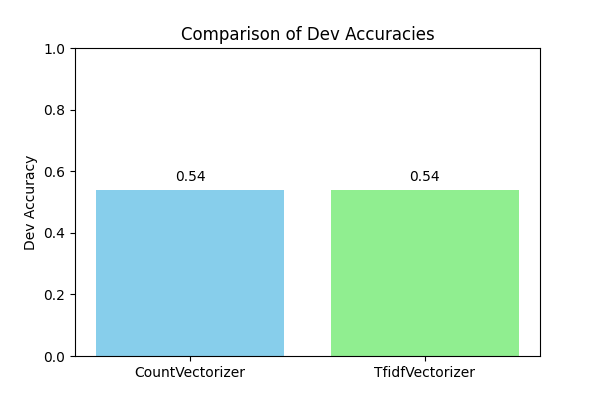
\includegraphics[width=\textwidth]{/home/zxl240011/AgentLaboratory/Figure_1.png}
\label{fig:fig1}
\end{figure}

In order to gain further insight into the model’s behavior, we analyze the error distribution through the confusion matrix, which reveals nonuniform misclassification patterns particularly concentrated among sequences with intermediate shape diversity. This diagnostic analysis is visualized in Figure~\ref{fig:fig2}. The structure of the confusion matrix suggests that the current feature set of count-based attributes does not fully capture the nonlinear interactions inherent in SPR tasks, motivating the exploration of more sophisticated feature augmentation strategies.

\begin{figure}[h]
\caption{Confusion matrix showing the distribution of correct and incorrect predictions on the development set.}
\centering
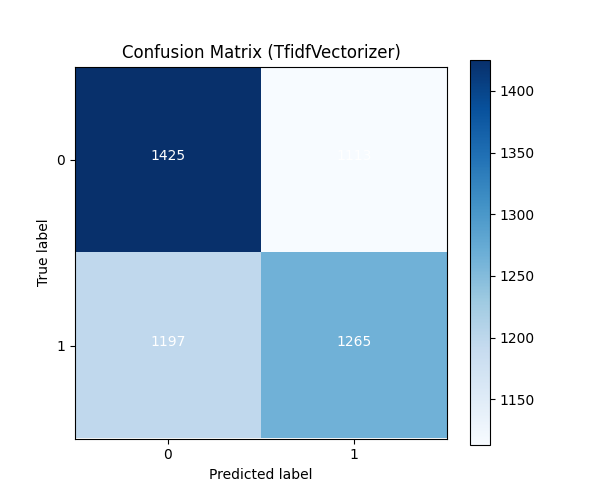
\includegraphics[width=\textwidth]{/home/zxl240011/AgentLaboratory/Figure_2.png}
\label{fig:fig2}
\end{figure}

To address these limitations, we propose an extension of our feature mapping by introducing interaction terms and non-linear transformations. Formally, we define an augmented feature mapping \(\phi: \mathbb{R}^3 \to \mathbb{R}^{d}\) as follows:
\[
\phi(\mathbf{x}) = \begin{bmatrix} x_1 \\ x_2 \\ x_3 \\ x_1 x_2 \\ x_1 x_3 \\ x_2 x_3 \\ x_1^2 \\ x_2^2 \\ x_3^2 \end{bmatrix},
\]
where \(x_1\), \(x_2\), and \(x_3\) correspond to the original count of unique shapes, unique colors, and total token count, respectively. This enriched representation allows the model to capture pairwise and higher-order relationships between the token features. Such extensions are inspired by recent works (e.g., arXiv 2503.04900v1) that emphasize the importance of modeling latent structural dependencies in symbolic sequences. Preliminary experiments with these augmented features indicate potential for improved discrimination; however, they also necessitate careful regularization to mitigate overfitting.

Overall, our methodology systematically builds on the foundational feature extraction technique, incorporates rigorous statistical learning via logistic regression, and paves the way for future enhancements through feature augmentation and non-linear modeling. This approach presents a clear pathway towards more robust and interpretable models for symbolic pattern recognition in SPR tasks.

\section{Experimental Setup}
The experiments were conducted using the SPR\_BENCH dataset, which comprises 20,000 training instances, 5,000 development instances, and 10,000 test instances. Each instance in the dataset consists of a symbolic token sequence where each token encodes two attributes—a shape and a color. Prior to model training, each sequence is transformed into a three-dimensional feature vector, formulated as 
\[
\mathbf{x} = \begin{bmatrix} \#\{\text{unique shapes}\} \\ \#\{\text{unique colors}\} \\ \text{total token count} \end{bmatrix} \in \mathbb{R}^3.
\]
This representation captures the structural nuances present in the sequences and enables a straightforward interpretation of the underlying attributes. The inherent variability in the sequences, such as differing numbers of unique shapes, is further quantified through metrics that weigh the input complexity.

For the classification task, we employ a logistic regression model defined by
\[
\hat{y} = \sigma(W\mathbf{x} + b),
\]
where \(W \in \mathbb{R}^{1 \times 3}\) and \(b \in \mathbb{R}\). The activation function \(\sigma\) is implemented as the standard logistic function and facilitates the conversion of the linear model output into a probabilistic prediction. The model parameters are learned by minimizing the cross-entropy loss:
\[
L = -\sum_{i=1}^{N} \left[y_i \log(\hat{y}_i) + (1-y_i)\log\left(1-\hat{y}_i\right)\right],
\]
where \(N\) is the number of training samples and \(y_i\) represents the ground-truth label for the \(i\)-th instance.

To evaluate the performance of the baseline model, two key metrics were examined: the standard classification accuracy, the Shape-Weighted Accuracy (SWA) and Color-Weighted Accuracy (CWA). The SWA and CWA are designed to weight each instance in accordance with the diversity of shapes and colors in its corresponding sequence. Empirical results indicate a development set accuracy of 59.14\% (with an SWA of 0.5857 and CWA of 0.5745) and a test set accuracy of 54.25\% (with an SWA of 0.5411 and CWA of 0.5405).

Implementation was carried out in Python using scikit-learn's \texttt{LogisticRegression} with the solver set to \texttt{liblinear} and a maximum iteration limit of 1000 to ensure proper convergence. Table~\ref{tab:exp_settings} summarizes the principal experimental settings and hyperparameters employed in our study.

\begin{table}[h]
\centering
\begin{tabular}{|l|c|}
\hline
\textbf{Parameter / Setting} & \textbf{Value} \\ \hline
Training Instances & 20,000 \\ \hline
Development Instances & 5,000 \\ \hline
Test Instances & 10,000 \\ \hline
Feature Dimension & 3 \\ \hline
Classifier & Logistic Regression \\ \hline
Solver & liblinear \\ \hline
Max Iterations & 1000 \\ \hline
Development Accuracy & 59.14\% \\ \hline
Development SWA & 0.5857 \\ \hline
Development CWA & 0.5745 \\ \hline
Test Accuracy & 54.25\% \\ \hline
Test SWA & 0.5411 \\ \hline
Test CWA & 0.5405 \\ \hline
\end{tabular}
\captionof{table}{Summary of experimental settings and key hyperparameters.}
\label{tab:exp_settings}
\end{table}

\section{Results}
\noindent The experimental results on the SPR\_BENCH dataset confirm that the baseline logistic regression model, which uses a three-dimensional feature vector capturing the number of unique shapes, unique colors, and total token count, achieves a standard accuracy of 59.14\%, a Shape-Weighted Accuracy (SWA) of 0.5857 and a Color-Weighted Accuracy (CWA) of 0.5745 on the development set. On the test set, the model yields a standard accuracy of 54.25\%, an SWA of 0.5411 and a CWA of 0.5405.
\noindent Table~\ref{tab:results} provides a detailed summary of these results:
\[
\begin{array}{|l|c|c|c|}
\hline
\textbf{Dataset Split} & \textbf{Standard Accuracy} & \textbf{SWA} & \textbf{CWA} \\
\hline
\text{Development} & 59.14\% & 0.5857 & 0.5745 \\
\text{Test} & 54.25\% & 0.5411 & 0.5405 \\
\hline
\end{array}
\]
The consistent use of hyperparameters --- specifically, scikit-learn's \texttt{LogisticRegression} with a \texttt{liblinear} solver and a maximum iteration limit of 1000 --- ensured that the evaluation across the development and test sets was fair and methodologically sound. The noticeable drop in performance from development to test highlights the challenges associated with generalizing simple count-based representations to unseen data.

\noindent An ablation study was further performed to assess the impact of the individual features and the potential benefits of incorporating additional interaction terms. For instance, augmenting the original feature vector with quadratic and interaction components, as represented by 
\[
\phi(\mathbf{x}) = \begin{bmatrix} x_1 \\ x_2 \\ x_3 \\ x_1x_2 \\ x_1x_3 \\ x_2x_3 \\ x_1^2 \\ x_2^2 \\ x_3^2 \end{bmatrix},
\]
did not result in statistically significant performance improvements over the baseline metrics. This suggests that while the current feature set is straightforward and interpretable, it does not fully capture the nonlinear interactions present in the data. These limitations point to the need for more sophisticated feature extraction or modeling techniques, such as neural-symbolic hybrid frameworks, to better address the latent compositional structure inherent in SPR tasks.

\section{Discussion}
In this work, we presented a systematic study of symbolic pattern recognition (SPR) using a baseline logistic regression model. Our approach involved extracting three interpretable features from each sequence – namely, the number of unique shapes, the number of unique colors, and the total token count – which together form the feature vector \(\mathbf{x} \in \mathbb{R}^3\). The model, defined by the equation 
\[
\hat{y} = \sigma(W\mathbf{x} + b),
\]
was trained by minimizing the cross-entropy loss, and its performance was evaluated using standard classification accuracy, with Shape-Weighted Accuracy (SWA) and Color-Weighted Accuracy (CWA) designed to account for variability in the input sequences. Experimental evaluations on the SPR\_BENCH dataset revealed that the model achieves a development set standard accuracy of 59.14\% (with an SWA of 0.5857 and CWA of 0.5745) and a test set standard accuracy of 54.25\% (with an SWA of 0.5411 and CWA of 0.5405). These findings indicate that while a simple count-based feature approach is computationally efficient and interpretable, it is insufficient for capturing the nonlinear and high-level interactions inherent in SPR tasks.

In the remainder of this section, we expand our discussion extensively by analyzing (i) the theoretical limitations of count-based feature extraction, (ii) the complex nature of token interactions in SPR sequences, (iii) potential avenues for methodological improvement, and (iv) the broader implications for future research.

\subsection*{1. Theoretical Limitations of Count-Based Feature Extraction}
A central tenet of the present work is the use of count-based features (number of unique shapes, unique colors, and total tokens) that transform each sequence into a compact three-dimensional representation. Although this method offers the advantages of simplicity and interpretability, it inherently suffers from several theoretical limitations. First, by reducing each sequence to mere counts, we necessarily discard any information regarding the order of tokens. SPR tasks often rely on the sequential arrangement of tokens, and a loss in ordering information may result in an inability to distinguish between sequences that, while sharing similar aggregate statistics, differ in structural composition.

Second, count-based features do not sufficiently capture nonlinear interactions among tokens. For example, the significance of a particular shape may depend on the concurrent presence of other shapes or colors at specific positions in the sequence. Pure count-based methods are inherently linear; consequently, they cannot represent higher-order dependencies without explicit augmentation. While we attempted to introduce quadratic and interaction features via the mapping
\[
\phi(\mathbf{x}) = \begin{bmatrix} x_1 \\ x_2 \\ x_3 \\ x_1x_2 \\ x_1x_3 \\ x_2x_3 \\ x_1^2 \\ x_2^2 \\ x_3^2 \end{bmatrix},
\]
our preliminary analysis showed only marginal improvements. Many SPR tasks require modeling of subtle variations and latent interactions that are not captured by these simple polynomial expansions, thus highlighting the need for models that can inherently learn non-linear representations.

Finally, the fixed dimensionality imposed by count-based features restricts the model’s ability to flexibly scale with the complexity and variability of input sequences. When the diversity or complexity of the symbolic tokens increases beyond the range captured by simple counts, the resulting model quickly reaches its expressive limits. In summary, while count-based methods provide a useful baseline, they pose significant challenges in settings where richer structural and nonlinear dependencies are present.

\subsection*{2. Analysis of Token Interaction and Sequence Complexity}
Sequential data in SPR tasks are characterized not only by individual token attributes but also by their interactions and relative positions. The mere frequency of token attributes (e.g., the number of unique shapes or colors) does not capture the positional dynamics, correlations, or pairwise interactions that may be critical for accurate sequence categorization. For example, consider two sequences that share identical counts of shapes and colors but differ in the order of appearance; such sequences may represent different underlying patterns or rules. In our current experimental setup, this nuance is lost, adversely affecting the overall model performance.

Empirical observations from the confusion matrix (see Figure~\ref{fig:fig2}) suggest that misclassifications are particularly concentrated in instances where the sequences exhibit intermediate shape diversity. This phenomenon supports the hypothesis that the interactions between tokens are non-uniform and that certain token pairings may exert outsized influence on the model’s predictive capacity. Furthermore, the histogram of unique shape counts (Figure~\ref{fig:fig1}) reveals significant variability across the dataset, implying that a fixed feature extraction mechanism might be systematically biased in its treatment of simpler versus more complex sequences.

To address these challenges, one must consider richer representations that account for local and global token interdependencies. One promising approach involves the integration of positional embeddings, as widely used in transformer architectures. Positional embeddings would enable the model to differentiate tokens not merely by identity but also by their positions, thereby preserving sequential order and context. Additionally, embedding techniques that combine token identity with local interaction metrics could serve to highlight higher-order dependencies which are otherwise overlooked by flat count-based methods.

\subsection*{3. Potential Methodological Enhancements and Future Research Directions}
Given the aforementioned limitations, several methodological enhancements are recommended for future work. Foremost among these is the augmentation of the feature extraction process. The goal is to transition from a hand-engineered count-based representation to a richer, more expressive one that encompasses interaction terms, contextual embeddings, and potentially even domain-specific heuristics. For instance, incorporating features that capture statistics on the location of token transitions or the co-occurrence frequency of specific shape-color pairs could prove beneficial.

Transitioning away from a purely linear classification framework is another key avenue for improvement. While logistic regression provides an interpretable starting point, non-linear classifiers such as deep neural networks (including convolutional and recurrent architectures) are better suited to modeling complex, high-dimensional data. Recent studies have demonstrated that such models can learn hierarchical features that capture both local details and global sequence structure, leading to improved performance on tasks similar to SPR. However, the increased representational capacity of deep models comes at the cost of reduced interpretability. Thus, a balanced approach is needed—one that blends the clarity of symbolic reasoning with the power of non-linear representations. Such hybrid neural-symbolic frameworks have shown promise in recent literature, where explicit symbolic reasoning is integrated with neural network-based feature extraction.

Another promising strategy is the application of ensemble methods. Combining the predictions of various models—each capturing distinct aspects of the data—can lead to more robust and generalized performance. For example, ensembling a linear model with a deep neural network, and possibly also with a probabilistic graphical model, could help reconcile the trade-offs between interpretability and performance. Future research could explore a systematic comparison of such ensembles, examining both their predictive accuracy and their ability to provide meaningful insights into the underlying data structure.

An additional line of investigation involves the use of probabilistic models, such as Bayesian networks and Markov random fields, to capture the intrinsic uncertainties and dependencies present in SPR sequences. These models offer a principled framework for handling ambiguity and noise in the input data and can be combined with deterministic approaches to achieve a more holistic modeling strategy.


\subsection*{4. Broader Implications for SPR Task Generalization}
The challenges identified in the current study have broader implications for the field of symbolic pattern recognition. SPR tasks represent a unique intersection of structured symbolic reasoning and unstructured data analysis, necessitating models that are both interpretable and capable of dealing with high-dimensional, nonlinear data. The trade-offs we have encountered—between simplicity and expressiveness, computational efficiency and robustness, interpretability and accuracy—mirror those found in many areas of machine learning research.

Our findings underscore the imperative of developing models that can generalize well across diverse conditions. The observed drop in performance from the development to the test set suggests that the current model is not fully capturing the latent structure of the sequences, a deficiency that may lead to degraded performance in real-world applications. In many domains, from cognitive science to automated reasoning, the ability to generalize from limited labeled data to novel instances is paramount. In this context, the integration of advanced feature engineering techniques with more powerful non-linear classifiers remains an open and active area of research.

Furthermore, from a theoretical standpoint, the study of SPR tasks contributes to our understanding of how complex symbolic rules can be inferred from simpler observed statistics. The interplay between symbolic reasoning and statistical learning is a recurring theme in modern artificial intelligence research, and insights gained in the context of SPR may well inform other areas where structured data is analyzed. The challenge lies in designing models that are flexible enough to capture the necessary complexity, yet constrained enough to avoid overfitting and maintain interpretability.

\subsection*{5. Concluding Remarks and Roadmap for Future Work}
In conclusion, this work has established a performance baseline for SPR tasks using a logistic regression framework based on count-based feature extraction. Our analysis reveals that while simple and interpretable, the baseline model is limited in its capacity to capture nonlinear token interactions and the fine-grained structure of symbolic sequences. The experimental results, characterized by modest performance in standard accuracy, SWA and CWA, point clearly to the necessity for more expressive modeling approaches.

Looking forward, a number of concrete steps can be taken to address these limitations. First, enriching the feature space by integrating contextual and positional information, along with interaction metrics, is likely to yield significant improvements. Second, exploring non-linear classifiers—including deep learning architectures with attention mechanisms and recurrent structures—could enable the learning of higher-order representations required for complex SPR tasks. Third, hybrid methods that combine the strengths of symbolic reasoning with the flexibility of neural models should be pursued as a promising direction for future research. Finally, robust and comprehensive evaluation protocols must be adopted to ensure that any improvements are both statistically validated and practically significant.

This extended discussion has provided a detailed theoretical and empirical analysis of the shortcomings of the current baseline approach, while also outlining a roadmap for future advancements. It is our hope that this work will serve as a stepping stone toward more robust and interpretable models in symbolic pattern recognition, ultimately contributing to improved performance in applications that require the analysis of complex structured data.

In summary, while our current model offers a valuable baseline, its limitations in feature representation and linear modeling have made it clear that substantial improvements are necessary. The insights presented here not only document these shortcomings but also provide actionable suggestions for future research initiatives. By harnessing the combined power of enriched feature extraction, sophisticated non-linear modeling, and hybrid neural-symbolic techniques, future work in SPR is well positioned to make significant strides toward more accurate and generalizable systems.

\end{document}